\documentclass[conference]{IEEEtran}
\IEEEoverridecommandlockouts
% The preceding line is only needed to identify funding in the first footnote. If that is unneeded, please comment it out.
\usepackage{cite}
\usepackage{amsmath,amssymb,amsfonts}
\usepackage{algorithmic}
\usepackage{graphicx}
\usepackage{textcomp}
\usepackage{xcolor}




%
\usepackage{graphicx}
\usepackage{cite}
\usepackage{picinpar}
\usepackage{amsmath}
\usepackage{amssymb}
\usepackage{url}
\usepackage{flushend}
%\usepackage[latin1]{inputenc}
\usepackage{colortbl}
\usepackage{soul}
\usepackage{multirow}
\usepackage{pifont}
\usepackage{color}
\usepackage{alltt}
%\usepackage[hidelinks]{hyperref}
\usepackage{enumerate}
\usepackage{siunitx}
\usepackage{breakurl}
\usepackage{epstopdf}
\usepackage{pbox}
\usepackage{breqn}
\usepackage{xfrac}
\usepackage{makecell}       % make cells inside tables
\usepackage{nomencl}        % Nomenclature package
\usepackage{multicol}		% Multiple columns
\usepackage{longtable}      % Table in multiple pages
%\usepackage{hyperref}       % hyperlinks
%\usepackage{cleveref}       % cross-referencing
%\usepackage{authblk}        % add affiliations
\usepackage{multicol}       % multiple columns
\usepackage{booktabs}		%For the table toprule midrule
%\usepackage{courier}
%\usepackage{subcaption}
%\usepackage{pdflscape}
%\usepackage{afterpage}
%\usepackage{pdfpages}
%\usepackage{xcolor}
%\usepackage[official]{eurosym}
%
%\newcount\Comments  % 0 suppresses notes to selves in text
%\Comments = 1
%\newcommand{\kibitz}[2]{\ifnum\Comments=1{\color{#1}{#2}}\fi}
%\newcommand{\bcr}[1]{\kibitz{black}{#1}} % color for review
%\newcommand{\bcb}[1]{\kibitz{black}{#1}} % color for review
%\newcommand{\bct}[1]{\kibitz{black}{#1}} % color for review
%



\def\BibTeX{{\rm B\kern-.05em{\sc i\kern-.025em b}\kern-.08em
    T\kern-.1667em\lower.7ex\hbox{E}\kern-.125emX}}


\begin{document}

\title{Conference Paper Title %*\\
%{\footnotesize \textsuperscript{*}Note: Sub-titles are not captured in Xplore and
%should not be used}
%\thanks{Identify applicable funding agency here. If none, delete this.}
}
%
%\author{\IEEEauthorblockN{1\textsuperscript{st} Benoit Couraud}
%\IEEEauthorblockA{\textit{James Watt School of Engineering}\\
%	 \textit{University of Glasgow, Glasgow (UK)} \\
%%\textit{name of organization (of Aff.)}\\
%%City, Country \\
%benoit.couraud@glasgow.ac.uk}
%\and
%\IEEEauthorblockN{2\textsuperscript{nd} Pierre-Jean Barre}
%\IEEEauthorblockA{\textit{Universite Cote d'Azur} \\
%\textit{IMREDD, Nice (FR)}\\
%%City, Country \\
%pierre-jean.barre@univ-cotedazur.fr}
%\and
%\IEEEauthorblockN{3\textsuperscript{rd} Roberta Pennucci}
%\IEEEauthorblockA{\textit{Universite Cote d'Azur} \\
%	\textit{IMREDD, Nice (FR)}\\
%	%City, Country \\
%	roberta.pennucci@univ-cotedazur.fr}
%\and
%\IEEEauthorblockN{4\textsuperscript{th} Yann Rozier}
%\IEEEauthorblockA{\textit{Universite Cote d'Azur} \\
%	\textit{IMREDD, Nice (FR)}\\
%	%City, Country \\
%	yann.rozier@univ-cotedazur.fr}
%\and
%\IEEEauthorblockN{5\textsuperscript{th} Sonam Norbu}
%\IEEEauthorblockA{\textit{James Watt School of Engineering}\\
%	\textit{University of Glasgow, Glasgow (UK)} \\
%	%City, Country \\
%	sonam.norbu@glasgow.ac.uk}
%\and
%\IEEEauthorblockN{6\textsuperscript{th}David Flynn}
%\IEEEauthorblockA{\textit{James Watt School of Engineering}\\
%	\textit{University of Glasgow, Glasgow (UK)} \\
%	%City, Country \\
%	david.flynn@glasgow.ac.uk} 


\author{\IEEEauthorblockN{Benoit Couraud$^{1,2}$, Pierre-Jean Barre$^{2}$, Roberta Pennucci$^{2}$, Yann Rozier$^{2}$, Merlinda Andoni$^{1}$, Sonam Norbu$^{1}$,\\  David Flynn$^{1}$}
	
	\IEEEauthorblockA{$^1$ James Watt School of Engineering, University of Glasgow, Glasgow (UK)\\
		Email: $\{$benoit.couraud,merlinda.andoni,sonam.norbu,david.flynn$\}$@glasgow.ac.uk\\
$^2$ IMREDD, Universite Cote d'Azur, Nice (France)\\
Email: $\{$pierre-jean.barre, roberta.pennucci, yann.rozier$\}$@univ-cotedazur.fr}
	%		\thanks{This work was funded by UK Engineering and Physical Sciences Research Council (EPSRC) through the CEDRI Project \cite{CEDRIProject}}
}




%\and
%\IEEEauthorblockN{7\textsuperscript{th} Merlinda Andoni}
%\IEEEauthorblockA{\textit{James Watt School of Engineering}\\
%	\textit{University of Glasgow, Glasgow (UK)} \\
%	%City, Country \\
%	merlinda.andoni@glasgow.ac.uk}
%\and
%\IEEEauthorblockN{5\textsuperscript{th} Given Name Surname}
%\IEEEauthorblockA{\textit{dept. name of organization (of Aff.)} \\
%\textit{name of organization (of Aff.)}\\
%City, Country \\
%email address or ORCID}
%\and
%\IEEEauthorblockN{6\textsuperscript{th} Given Name Surname}
%\IEEEauthorblockA{\textit{James Watt School of Engineering, University of Glasgow, Glasgow} \\
%	%\textit{name of organization (of Aff.)}\\
%	%City, Country \\
%	david.flynn@glasgow.ac.uk}
%}

\maketitle

\begin{abstract}
	Most of western countries have successfully deployed Smart Meters and are now in a phase of exploration to regulate and leverage the use of smart meter data. In France, the Linky smart meter provides data locally to the end-users in close to real-time, whereas it also makes 30 minutes data available to third party servers on the following day, which is inappropriate for operational applications.  In this work we detail the design of a full plug and play solution named Linky TIC Reader (LTR) to locally collect data from the  French smart meter and make it available to  end-users or to third party energy services providers in close to real time. Although many products to read Linky TIC output are already commercialised, they are usually externally supplied, unlike the LTR described in this work. This  will democratise access to an interoperable solution to control  and automatically limit households' overall consumption at a low cost and for all distribution board configurations.
	%, and will support the shift towards electric heating and transport by enabling the disconnection of flexible assets such as heaters and electric vehicle chargers before the main circuit breaker cut off the entire household in case of power consumption excess. 
	Finally, this article describes several potential applications of the data collected by the LTR, such as load management, non-intrusive load monitoring and load forecasting. 
\end{abstract}

\begin{IEEEkeywords}
	Linky, load management, smart grids, smart meter
\end{IEEEkeywords}

\section{Introduction}
The energy transition requires the shift of several residential usages for electric technologies, such as electric vehicles and heat pumps to decarbonise transport and heat respectively \cite{RTEScenario:techrep}. Similarly, the increase of energy prices and especially gas prices has led many buildings, shared properties and homes to shift from gas based heating systems to electric heaters. However,   the electric distribution  grid cannot always be reinforced in the short term in gas heating based  properties that were originally designed for minimal use of electric power. In this case, end-users are often not allowed to increase their maximum power subscription, and the transition for electric heating requires them to switch off some of their electric appliances to prevent the electric meter to instantly disconnect the entire household due to an excess of consumption compared to the maximum power subscribed. Furthermore, national power production limitations might also require electric usage to be reduced at specific times, as it advised by external signal such as Ecowatt in France \cite{ecowatt:website}. This demonstrates the importance of flexibility at a residential level. Such flexibility can be provided following different use cases and levels of decision making. First, the distribution system operator (DSO) can leverage the smart metering infrastructure to disconnect  households that are in a highly constrained location. Second, aggregators or energy services providers can use smart devices at the households premises to provide services to the end-users such as house overall power limitation through smart heating \cite{voltalis:website} and smart charging \cite{chargeangels:website} to ensure a smooth integration of these additional electric appliances to residential households. Third, flexibility can be controlled directly by the end-users without any third party's intervention, in which case it can be done manually or automatically through smart devices and IoT (Internet of Things) based solutions. All these levels of flexibility that aim to limit the power consumption of a household require the use of a device such as a smart meter to monitor and communicate the house's overall power. 

In this paper, we focus on the case of France, that has already deployed more than 35 millions of its smart meter \textit{Linky}, which has positioned this smart meter project as one of the largest and most comprehensive globally. As France is now working on regulations of smart meters' data usage \cite{cre:website}, this paper first aims to describe low-tech solutions to collect smart meter's real time data. Second, the paper aims to discuss the potential benefits and usage of Linky's real-time data, especially in the context of residential flexibility procurement as required by the energy transition. 
The paper  is organised as follows: Section \ref{section:needs} describes the current context and need for flexibility at households level. Then, Section \ref{section:solution} proposes a solution to collect the French smart meter real-time data and make available to the end-users or to third party energy services providers. Finally, Section \ref{section:experiments} discusses the limits of this solution and of the quality of the data collected, especially related to energy and non-energy services.

\section{Smart Meter enabled Flexibility}
\label{section:needs}

\subsection{Needs for Residential Flexibility}
The energy transition will  result in an electrification of transport and heat, which will strongly impact the distribution network. Although some locations of the low voltage network will not require any reinforcement to supply all these new loads such as electric vehicles (EV) and heat pumps (HP), some other places will be impacted in terms of voltage excursion and excessive network cables heat at specific times of the day. To visualise these impacts, we ran a power flow study on the standard European Low Voltage network feeder \cite{IEEE:PESTestFeeder} for different deployment rates of EVs and HP. We randomly allocated real households, EVs and HP load profiles at the houses locations defined in the network from \cite{IEEE:PESTestFeeder} and computed the resulting voltage and electric current levels for more than 120  simulations with random geographical allocation of loads. Households and EVs load profiles are minutely data that come from the UK  largest smart local energy system demonstrator in the Orkney Islands, named the Responsive FLEXibility (ReFLEX) project that monitored over 140 EVs; whereas HP load profiles came from the large scale trial "Renewable Heat Premium Payment Scheme" \cite{RHPP} that monitored hundreds of heat pumps with a granularity of 2 minutes. The average daily number of minutes with voltage excursions (below the lower voltage limit) was recorded and is displayed in Fig. \ref{Fig:voltage_excursion} as a function of the deployment rate of EV and HP. It shows that the low voltage network of neighbourhoods with full deployment of electric heating and EVs, might experience more than one hour per day with local voltage constraints. These constraints could either be solved by expensive grid reinforcement, or by residential flexibility coordinated by a third party (DSO or an aggregator). 

\begin{figure}[h]
	\centering
	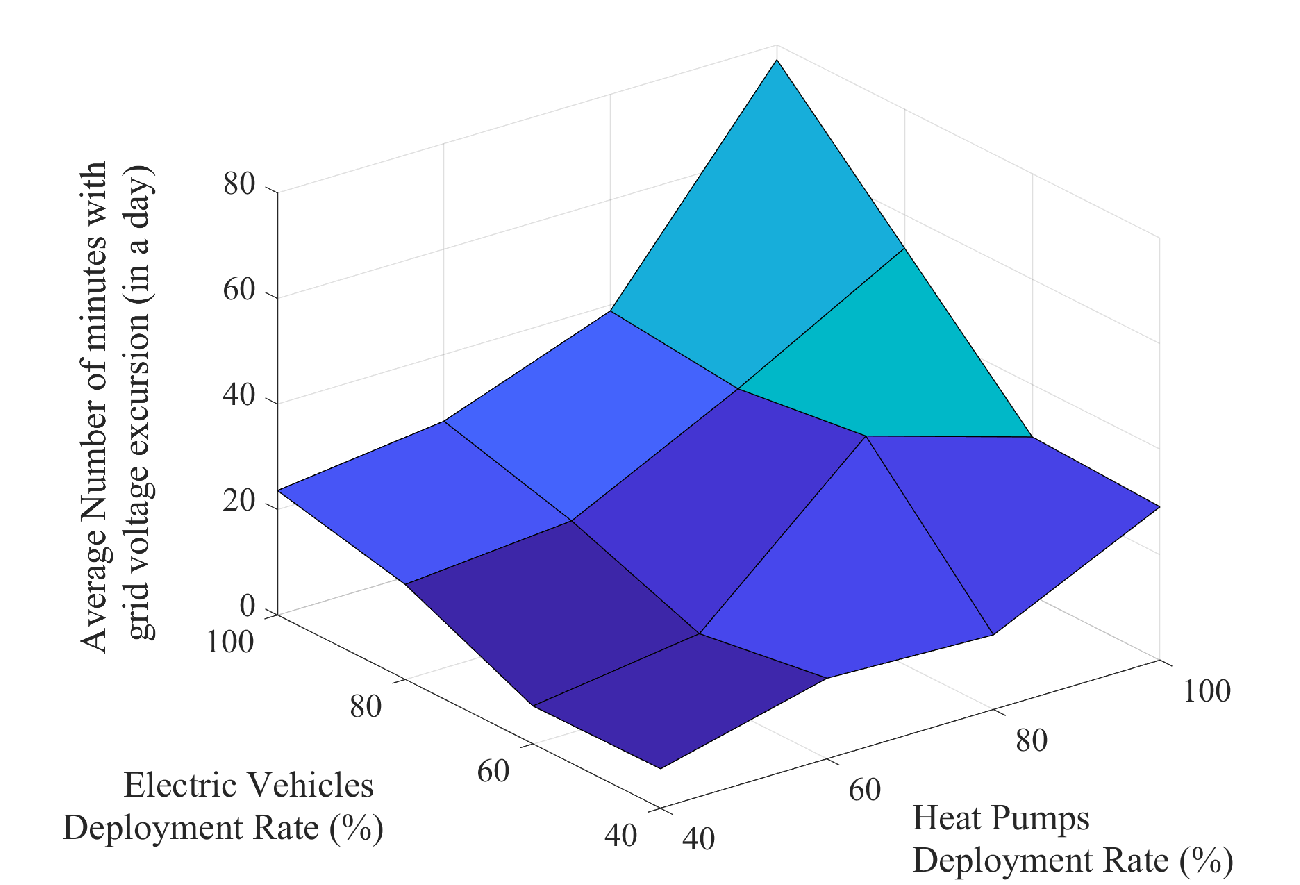
\includegraphics[width=0.75\columnwidth]{Images/ReFELX_EV_HP_Impact_Map2.pdf}
	\caption{Simulated average number of minutes in a day with Low Voltage network voltage excursions in a European neighbourhood.}
	\label{Fig:voltage_excursion}
\end{figure}

Furthermore, the recent increase of gas price in many countries has led buildings to shift from gas heating to electric heating. This shift has considerably increased some households' loads at peak time, and might require an increase of maximal power subscription to prevent the smart meter's circuit breaker to cut-off households. However, such maximal power subscription increase  is usually not  possible in the case of old infrastructures as it is usually the case in western countries. Therefore, several households have experienced instantaneous power cut due to excess of load. This can be seen in Fig. \ref{Fig:load_example} where an apartment with a 6kVA subscription was disconnected from the grid at 18:44 by the smart meter circuit breaker due to a power consumption excess from electric loads including water storage heater, space heaters and cooking plates. A similar issue could also be faced by households acquiring an EV, that entails an additional nominal load for charging power ranging from 3.7kW to 7.2kW (as shown in the purple curve of Fig. \ref{Fig:load_example}), which also might lead to power cut if an increase of maximum power subscription is not possible. Such situations could be avoided through the use of households flexibility solutions leveraging real-time smart meter data. 

\begin{figure}[h]
	\centering
	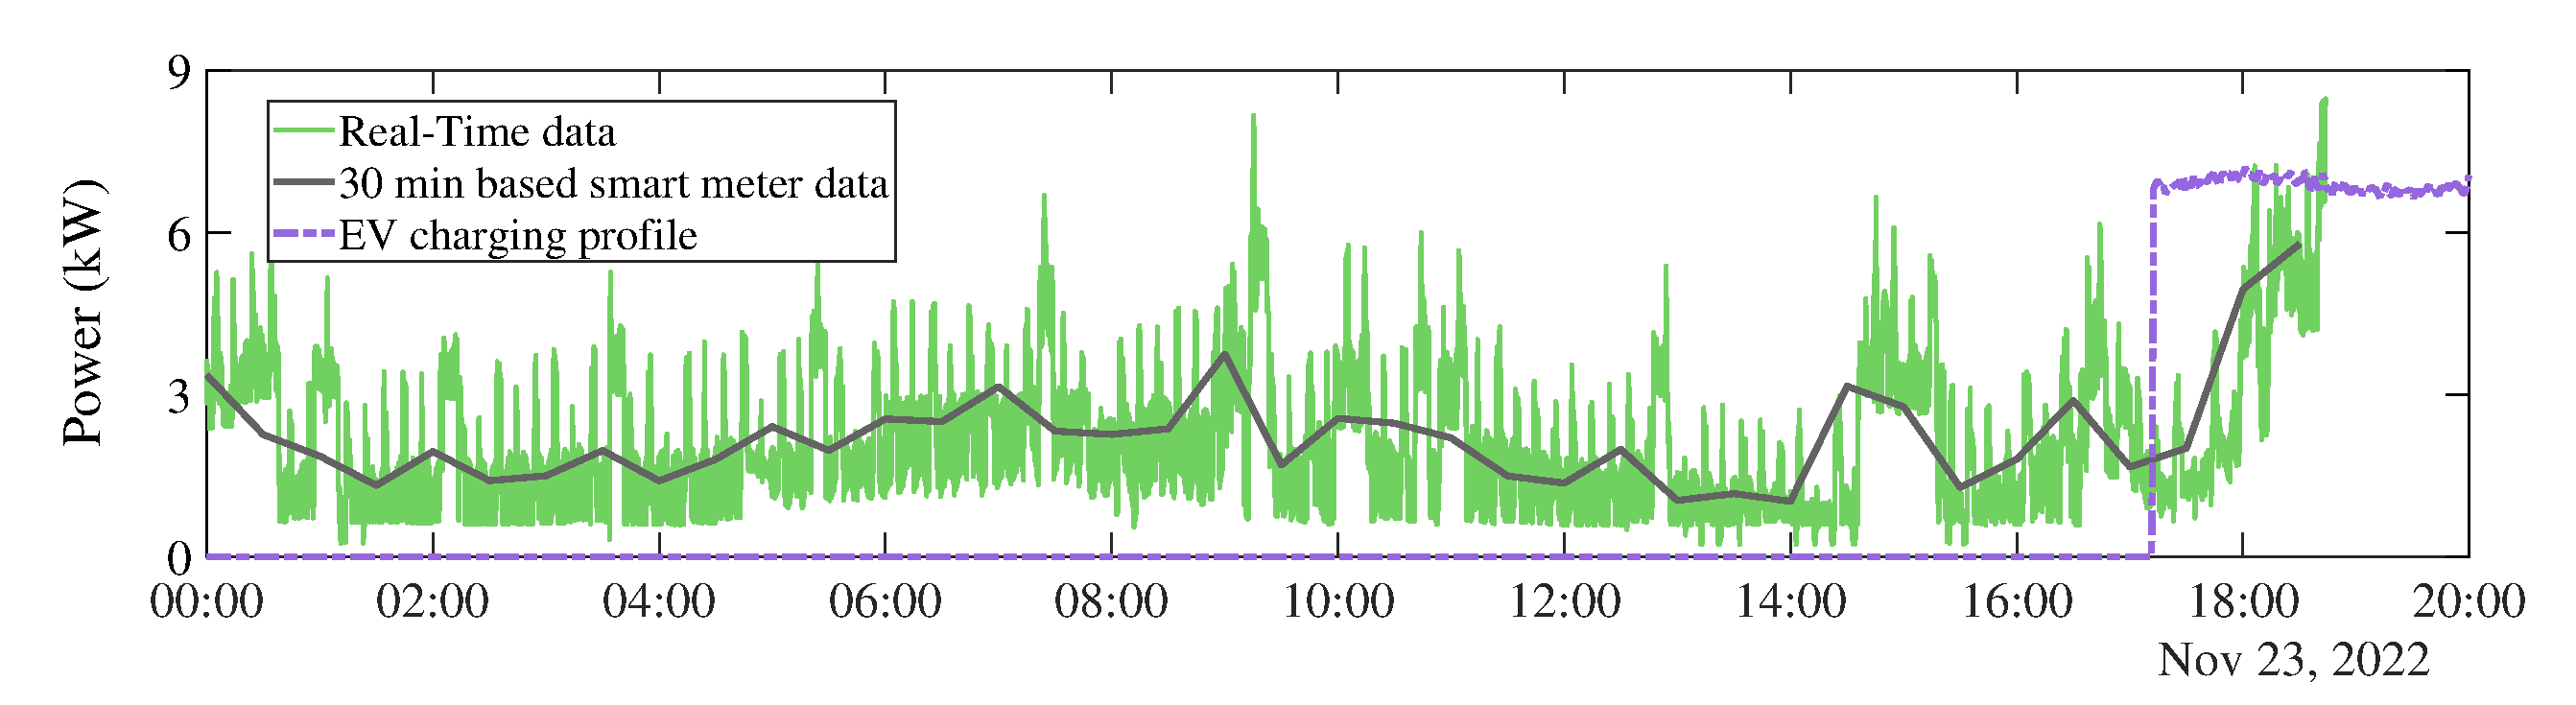
\includegraphics[width=1\columnwidth]{Images/load_curvesEV.pdf}
	\caption{Example of an EV charger load curve and of a winter's household electric load with a power subscription of 6kVA, and disconnection at 18:44.} % An example of real EV load is also shown for information purposes.}
	\label{Fig:load_example}
\end{figure}

\subsection{French Smart Meter Characteristics}
The French smart meter provides two types of data that are shown in Fig. \ref{Fig:load_example}. One that is automatically sent at a remote concentrator of the French DSO through power line communication \cite{IEEE:LinkyInfrastructure}, and that is made available through websites or APIs (Application Programming Interface) to the end-users on the following day, with a 30minutes time interval, making it inappropriate for use in operational decisions for electric flexibility. On the other hand, the other type of data proposed by the French smart meter is available locally, through connectors of the smart meter named the TIC (Tele-Information Client) and visible in Fig. \ref{Fig:dongle_Linky}, at a time granularity below 5 seconds, but requires an additional electronic device to read this real-time data and send it to a back-end that would be able to inform the end-users or a smart appliance of a load power excess. This additional electronic device must be able to decode the TIC data sent locally by the smart meter through its electronics connectors, and can be supplied directly by the smart meter. However, for power supply of such electronic device, the French smart meter only provides an AC signal of 6$V_{rms}$ at 50kHz with a minimum power of 130mW \cite{Enedis:Linkyspec}, which is very low to supply an electronic device that aims to send data in real-time to a web service through an internet or a LoRa connection. 

This section demonstrated the need for a precise and real-time monitoring of households' load consumption in order to enable a necessary local or coordinated flexibility aiming to support the energy transition and electrification. In the case of the French infrastructure, it was shown that such monitoring can be done by the smart meter Linky, but it requires the integration of an electronic device that can be supplied by the smart meter itself, but with great constraints. The next section will describe the design of such an electronic device aiming to automatically read the household's power consumption from the smart meter, send data to third party services if needed, and provide control of local flexible assets such as heating devices or electric vehicles.


\section{Solution for French Smart Meter Data Collection}
\label{section:solution}
This section describes the details of a Linky TIC Reader (LTR) supplied directly by Linky. The main constraints faced when designing such a solution are the low power supply available at the Linky connection to supply the LTR, and the space constraints that we have to meet to integrate such a device into Linky's casing. Indeed, the power supplied by Linky for a LTR is slightly greater than 130mW, whereas the minimal power requirement to send any message is between 400 and 560mW over a few seconds for wifi protocol, and between 60 and 400mW for LoRa communication. Therefore, the main approach for a LTR is to store energy in a large capacitor, and to first power up the LTR when there is enough energy to read Linky's data. Then, when the energy is greater and large enough for transmission, the LTR can send data to a third party web service. It is therefore necessary to consider four main operations: first, the charging phase of the capacitor, that occurs every time the other operations have emptied the capacitor, second the recording phase, that aims to read data from the smart meter. third, the action phase, that consists in switching on or off flexible assets directly connected to the LTR in case of high household power consumption, and finally the communication phase that sends data to a remote third party for energy or non-energy services. 

\subsection{Architecture of the LTR}
The LTR is composed of 4 main elements. The power supply, the demodulation, the communication and control, and the actuator modules.   The links between all of these elements and their schematic is proposed in Fig. \ref{Fig:schematic}. Because the wifi constraints are higher than for other Radio-Frequency protocols, Fig. \ref{Fig:schematic} and the rest of the paper focus on a Wifi version of the LTR, that only applies to households for which the smart meter is at an acceptable range of the internet box. However, everything is fully replicable in a LoRa configuration. Each one of the four elements presented in Fig. \ref{Fig:schematic} are described in the next subsections.



\begin{figure}[h]
	\centering
	\includegraphics[width=1\columnwidth]{Images/schematic.pdf}
	\caption{Global schematic of the LTR.}
	\label{Fig:schematic}
\end{figure}



\subsection{Demodulation Module}
The demodulation module aims to demodulate the signal that is made available by the Tele-information Client (TIC) connector of Linky smart meter. It adopts a very well-known optocoupler based architecture that is already available to purchase on the market, and will therefore not be described here. We highlight however that there are two versions of the French smart meter: one that communicates at 1200bps, and another one at 9600bps. Depending on the version, the value of the demodulator resistor at the output of the optocoupler should be changed from 22k$\Omega$ to 12k$\Omega$ respectively, as it is shown in Fig. \ref{Fig:schematic}. 

\subsection{Actuator}
The actuator aims to connect or disconnect the load depending on the household's power consumption. It consists of a latching relay similar to the one in \cite{adafruit:latchingrelay} with two coils in order to limit the power consumption from the control module. This way, the control module must dedicate one output pin to set the relay for a few miliseconds (i.e. energize one of the two coils of the relay) in order to supply a load that would be connected to the relay, and another output pin to unset the relay. Small loads can directly be connected to the relay. Otherwise, the use of an intermediary circuit breaker as it is done for peak/off-peak hours circuit breakers \cite{schneider:circuitbreaker}.

\subsection{Power Supply Module}
Although it is possible to directly supply the demodulation and communication modules using an electric plug from the house distribution board, this paper focusses on the design of an integrated solution that directly powers from the smart meter and that would fit in any household, either those with the smart meter in the range of a Wifi connection, or those out of range, that can then use LoRa or GSM connection, based on the same operation principles described in this paper. The power supply aims to rectify the AC power available, to charge a supercapacitor that acts as an energy tank and to connect this supercapacitor to the rest of the circuit (i.e. the demodulation, communication and actuator module) through the MOSFET $Q_1$ (right side of Fig. \ref{Fig:schematic}) when it is enough charged. The indication that the supercapacitor is charged enough is given by its voltage ($V=\sqrt{\frac{2E}{C}}$), which can be used to trigger the supply or cut off of the rest of the circuit.
 The complexity of this task  lies in the fact that due to the small amount of power available from Linky, when the capacitor achieves a voltage that is considered as large enough to supply the communication circuit for a few seconds, this voltage will decrease rapidly once this communication module is connected, which might then switch off again the communication module due to a lower voltage, unless an hysteresis control loop is implemented. Indeed, the idea for this power supply module is to switch on MOSFET $Q_1$ at a high voltage of the supercapacitor $C_1$, and to keep it switched on until the voltage of $C_1$ is considerably lower. Although a Schmitt trigger could meet this requirement in theory, it does not work correctly in practice as the trigger's supply voltage (i.e.  $V_1$, the voltage at $C_1$ output) is not stable because the Schmitt trigger input is derived from (proportional to) the supply voltage. Therefore, we chose to use a microcontroller $U_1$  to control the voltage of the hysteresis and to control the switching of  $Q_1$ and the supply of the rest of the circuit.  The microcontroller implements the following logic: if the capacitor voltage has been above 4.5V for at least  20 consecutive cycles (with a low frequency of 1MHz), the switch $Q_1$ is switched on. This connects the ground voltage level of the communication and control module with the ground level of  $V_1$, which will supply the communication and control module. The switch  $Q_1$ is kept switched on  until the voltage $V_1$ drops below a threshold of 4.1V for at least 200 cycles. As the microcontroller is directly supplied by $V_1$, the $C_1$ capacitor voltage, the voltage measurement is done by an analog input of $U_1$ that measures the voltage at the 3.3V Zener diode $D_1$ which is triggered by a digital output pin of $U_1$ to save energy. The total cost for a single  power supply module is below 13€. 
 
 \subsection{Communication and Control Module}
 In normal operation, the communication module of the LTR achieves three main purposes. First, it wakes up from sleep mode and reads  Linky data made available at the output of the demodulation module and stores it in EEPROM memory before going back to sleep mode to save energy. Second, it takes the decision to switch on or off the actuator (flexible electric appliances such as water storage heater of EV) based on the instant power consumption  measured by the smart meter. Indeed, if the power consumption is greater than a predetermined threshold given by the household's power subscription, it is urgent to switch off flexible appliances. Also, if the power consumption is above a given threshold, the communication module will send this information through WIFI or LoRa to a third party web service that can then switch on or off smart appliances remotely, such as EV chargers for example. Finally, if the voltage $V_1$ is high enough, the communication module connects to a registered WIFI network and sends 	all the previously recorded data to a remote server (e.g. third party web service).  
 
 Before achieving this normal operation mode, the communication module must be configured in order to connect to the right WIFI SSID and to store the web addresses to which data should be sent. This is done at the initialisation phase of the LTR by having the communication module set up in Access Point mode with an interval web server stored until it is able to connect successfully to another existing WIFI. 
 
 In order to propose an open source design that anyone could reproduce and install at their household, we worked with the compact, fully democratised and easy to use ESP8266 based WEMO D1 mini Lite boards, that can be purchased for less than 10€. One of the main advantage of such boards is that many libraries have been developed to help the implementation. More specifically, such boards have all the Transport Layer Security protocols available in dedicated libraries. Therefore, using these boards allow an easy implementation of security layers to safely connect to https servers. In the case of ESP8266 based modules, we have configured a Wificlient secure instance to set trust anchors using real https  certificates delivered by a root SSL certification authority. The advantages and disadvantages of using secure connection to remote servers is discussed in Section \ref{section:experiments}.
 
 
 \begin{figure}[h]
 	\centering
 	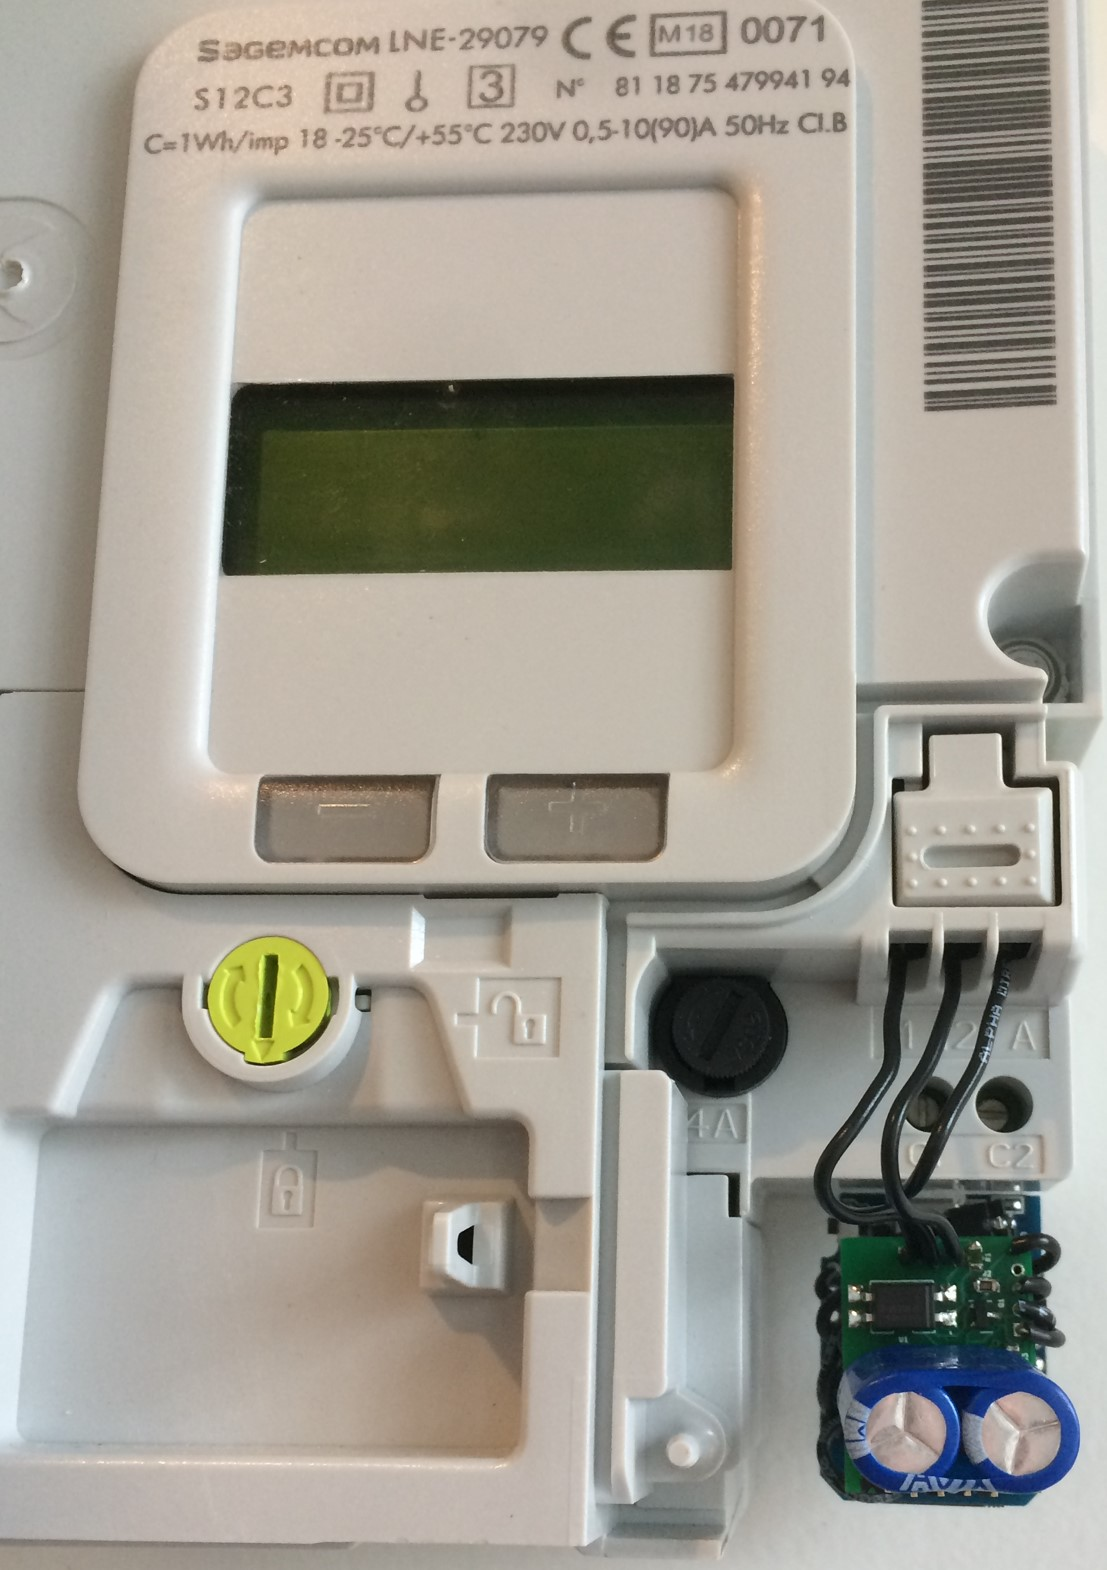
\includegraphics[width=0.5\columnwidth]{Images/dongle_Linky.jpg}
 	\caption{Integration of the WIFI based Linky TIC Reader (LTR) device for Linky local data collection and transmission to third party energy services.}
 	\label{Fig:dongle_Linky}
 \end{figure}
 
 
 
 The final result of an LTR implementation is displayed in Fig. \ref{Fig:dongle_Linky}, with a single unit price below 30€. All the schematics and codes to reproduce this Linky TIC Reader (LTR) are  available as open source documentation from the github repository referenced in \cite{github:LTR}.





\section{Use of LTR for Energy Services}
\label{section:experiments}
In this section, we describe the experimental results of the LTR testing phase, and discuss several usages this device. 
\subsection{Experimental results}
The LTR was implemented, tested and deployed in several households for a period of over 6 months. Fig. \ref{Fig:load_example} displays the data captured by one of the LTR in green, and in grey is displayed the associated smart meter data. The main learnings from this implementation mostly concern the time interval between two consecutive data transmission, as it is the only characteristics that depends on the environment (power available at the smart meter's end). Table \ref{Table:securityimpact} shows the time interval between two consecutive data sent to a remote server. We can see that because of the low power supply and the high energy requirements for the communication module to send data, the time between  two consecutive transmission of data by the LTR is always above 19 seconds. However, we also note that for custom applications, it is possible to send data as a bunch, instead of one data per transmission. However, for third party services, the data sent might have to be single and can be the average of all recorded values since the last transmission.

Also, we can differentiate the case in which a secure connection was established with the server through https, and the case without any security considerations. 

%
		\begin{table}[h]
	\caption{Impacts of security layers on LTR data transmission.} % frequency.} 
	\label{Table:securityimpact}
	\small % text size of table content
	\centering % center the table
	\begin{tabular}{lccc} % alignment of each column data
		\toprule[\heavyrulewidth]\toprule[\heavyrulewidth]
		\textbf{Operation mode} &  \multicolumn{3}{c}{ \textbf{time interval between 2 transmissions }} \\

		\textbf{} &  mean (s) &  max (s) &  min (s)\\		
		\midrule
		with security layers & 54.6 & 140 & 20 \\ 
	without security  & 33 & 68 & 19 \\ 
		\bottomrule[\heavyrulewidth] 
	\end{tabular}
\end{table}
%
%mean 54.6   max  140  min  20
%mean 33 max 68 min 19

Because of the required security handshake and encryption, the energy consumed by the LTR to send data in the case of secure connection is much higher than for a simple http connection. As a result, it takes more time for the LTR supercapacitor to retrieve an acceptable voltage level allowing the LTR to send data again. Therefore, a lower frequency in data collection is the price to pay for a secure connection with encrypted data and effective authentication of the device and the server. In the rest of the paper, we discuss the potential impacts on energy and non-energy services carried out by third parties using this data at a lower frequency. 
 
 
 \subsection{Use cases for LTR data}
LTR data is data from the smart meter that is made available at a much higher frequency than the DSO operator (around 1min data for the LTR against 30 min data for the DSO services). However, it is not full real-time data as remote servers will receive data only once every 30-55 seconds. We discuss here the potential use of such data, following the list of applications proposed in \cite{IEEE:ReviewSmartMeterData}.
\subsubsection{Load Analysis }
Load analysis mostly consists in the identification of issues in the load profile of a households (bad data, non-technical loss, profiling). Using high frequency data, it is also possible to provide services in a new application, which consists in the identification of residential flexibility procurement. Residential flexibility settlement require an aggregator to compute the flexibility effort (i.e. the flexibility delivered compared to a baseline). It currently consists in the comparison of an average consumption  (based on 30min data) over several days prior to the time of delivery, called the baseline, and the actual consumption \cite{ESO:BaselineP376}. Adding capabilities such as the ones described in Section \ref{section:NILM} could help to identify actual flexibility efforts based on assets switching and not only reduction in power consumption.


\subsubsection{Load Management}
LTR can be used to identify the need to reduce an household's power consumption, and then to switch off one of the flexible assets (heating appliances, EV chargers, ...) either by directly controlling the assets, as described in Fig. \ref{Fig:schematic}, or remotely by sending the request to a remote server able to control flexible assets. In this case, it is possible to send such request as soon as a high power consumption has been read from the Linky, without waiting for the supercapacitor $C_1$ to be full enough.


\begin{figure}[h]
	\centering
	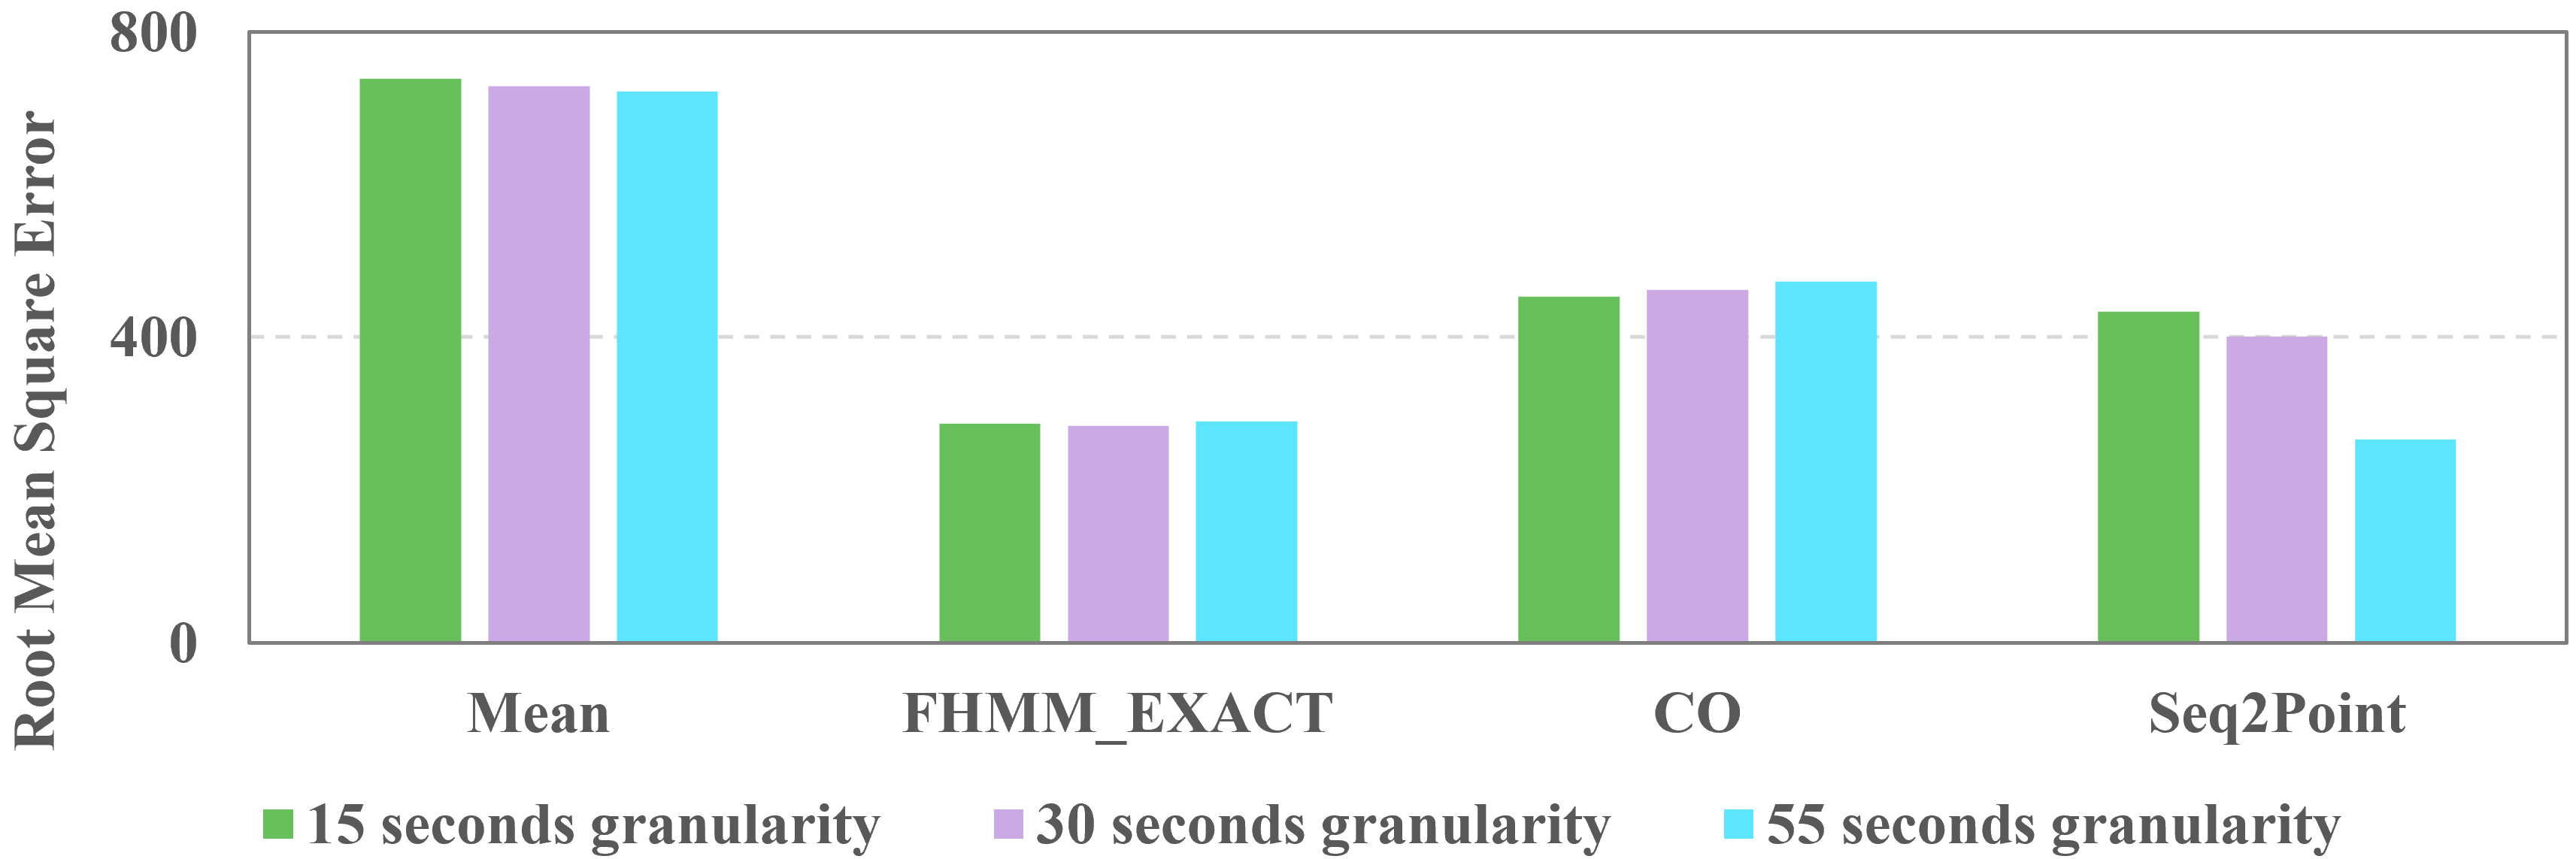
\includegraphics[width=0.85\columnwidth]{Images/NILMComparison}
	\caption{Comparison of  RMSE for 4 state of the art NILM algorithms used for different frequency of data transmission (15, 30 and 55 seconds).}
	\label{Fig:NILMComparison}
\end{figure}

\subsubsection{Non-Intrusive Load Monitoring}
\label{section:NILM}
Non-intrusive Load Monitoring (NILM) consists in the identification of appliances' switching (on or off) based only on the mains' measurement. It usually requires high frequency resolution monitoring data (seconds to sub-second). We implemented state of the art NILM algorithms to compare the capability to identify appliances with LTR data with and without security layers.  Fig. \ref{Fig:NILMComparison} shows the Root Mean Square Error (RMSE) for identification of a water storage heater in an apartment in October based on 2 weeks of data with a period of calibration with only the water heater storage appliance connected to the mains.  We can see that for each algorithm, the identification error is similar for all data transmission time except in the case of the Sequence to Point algorithm for which 55 seconds between two data transmission provided even better results in our case than any other algorithm used with 15 seconds data granularity. This demonstrates that if the TLR was to be used for NILM purposes, the addition of security layers would a priori not reduce the efficiency of the disaggregation. However, the calibration process might not be compatible with residential use cases.

\subsubsection{Load Forecasting}
Finally, LTR can be used for load forecasting purposes. It was reminded in \cite{IEEE:ReviewSmartMeterData} that load forecasting algorithms for individual households provide very low accuracy, and thus high Mean Absolute Percentage Error, especially compared to the case of aggregation with many other households. In this paper, we leverage LTR data to determine the impact of data aggregation in time (from the energy consumed per hour to the energy consumed over 24h) on the accuracy of load forecasting achieved by the efficient k-Nearest Neighbours algorithm.

\begin{figure}[h]
	\centering
	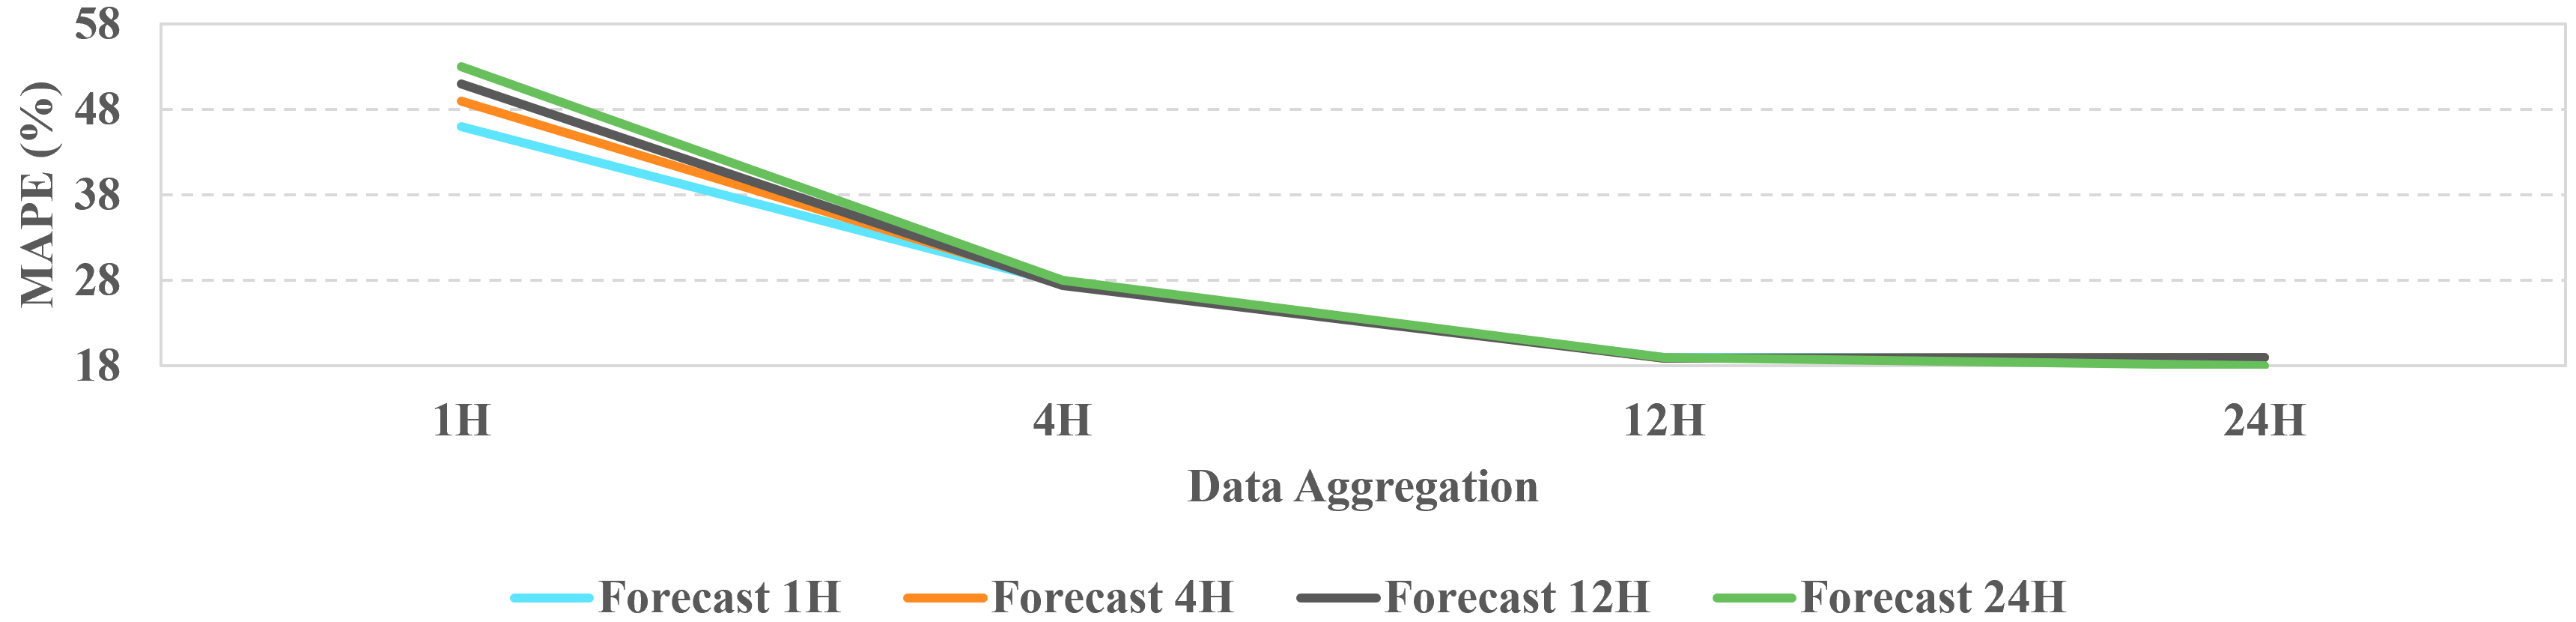
\includegraphics[width=1\columnwidth]{Images/ForecastAccuracy.png}
	\caption{MAPE accuracy for prediction of a single house load profile for different levels of data agregation.}
	\label{Fig:ForecastAccuracy}
\end{figure}
 Fig. \ref{Fig:ForecastAccuracy} shows that the accuracy increases considerably with the aggregation of data in time. This outcome can be used when designing a local energy market, as it shows that individual households' load forecasts with aggregation below 12hours might lead to very high forecast errors for the corresponding market time interval, and thus to penalise the end-users.

 




\section{Conclusion}


\section*{Acknowledgment}

The preferred spelling of the word ``acknowledgment'' in America is without 
an ``e'' after the ``g''. Avoid the stilted expression ``one of us (R. B. 
G.) thanks $\ldots$''. Instead, try ``R. B. G. thanks$\ldots$''. Put sponsor 
acknowledgments in the unnumbered footnote on the first page.



% References

\bibliographystyle{Bibliography/IEEEtranTIE}
\bibliography{Bibliography/IEEE_biblio.bib}\ %IEEEabrv instead of IEEEfull



%
%\begin{thebibliography}{00}
%\bibitem{b1} G. Eason, B. Noble, and I. N. Sneddon, ``On certain integrals of Lipschitz-Hankel type involving products of Bessel functions,'' Phil. Trans. Roy. Soc. London, vol. A247, pp. 529--551, April 1955.
%\bibitem{b2} J. Clerk Maxwell, A Treatise on Electricity and Magnetism, 3rd ed., vol. 2. Oxford: Clarendon, 1892, pp.68--73.
%\bibitem{b3} I. S. Jacobs and C. P. Bean, ``Fine particles, thin films and exchange anisotropy,'' in Magnetism, vol. III, G. T. Rado and H. Suhl, Eds. New York: Academic, 1963, pp. 271--350.
%\bibitem{b4} K. Elissa, ``Title of paper if known,'' unpublished.
%\bibitem{b5} R. Nicole, ``Title of paper with only first word capitalized,'' J. Name Stand. Abbrev., in press.
%\bibitem{b6} Y. Yorozu, M. Hirano, K. Oka, and Y. Tagawa, ``Electron spectroscopy studies on magneto-optical media and plastic substrate interface,'' IEEE Transl. J. Magn. Japan, vol. 2, pp. 740--741, August 1987 [Digests 9th Annual Conf. Magnetics Japan, p. 301, 1982].
%\bibitem{b7} M. Young, The Technical Writer's Handbook. Mill Valley, CA: University Science, 1989.
%\end{thebibliography}

\end{document}
